\documentclass[a4paper]{article}

\usepackage[english]{babel}
\usepackage[utf8]{inputenc}
\usepackage{amsmath}
\usepackage{graphicx}
\usepackage[colorinlistoftodos]{todonotes}
\usepackage{natbib}
\usepackage{fixltx2e}
\usepackage[version=3]{mhchem}
\usepackage{float}



\bibliographystyle{agsm}

\title{Devonian Granite types in Victoria and their origin}

\author{James Stone - 761353}

\date{October 2015}

\begin{document}
\maketitle
\newpage

\begin{abstract}
The abstract.
\end{abstract}

\section{Introduction}

The Granites of Victoria are situated almost totally within the Lachlan Fold Belt, which in turn is part of the larger Tasman Fold Belt System, See Figure~\ref{fig:VicStructuralZones} and  Figure~\ref{fig:VicMapRockTypes}. The regional geological environment through which the Devonain granites intruded is one of alternating deep and shallow marine sedimentary rock deposited during the Ordovician and Silurian along the continental edge of the older Delamerian Fold Belt to the West.

Classification of granites by origin was originally pioneered by Chappell and White in 1974 and was initially specific to the Berridale (I type) batholith and the Kosciuszko (S type) batholith in Southern New South Wales. Whilst this was regionally limiting, their research and conclusions have largely stood the test of time and have since been applied with success to describe granite emplacement mechanisms throughout the Lachlan Fold Belt and across other granitic regions of the world.

\section{Body of Essay}
\label{sec:Body of Essay}



Granites can be classified into two major types; the S-Type and the I-type. \cite{BWChappell}
This classification distinguishes the granites by their source and utilises both geochemical and petrological characteristics. It is accepted that the present day features of granites form an "image" of their source rocks, \cite{BWChappell} (Chappell, 1979), acknowledging that fractionation of the magma body often occurs. The more homogeneous the batholith, the more it accurately reveals its origins. 

The more mafic the granite, the closer it resembles its source rocks, and the easier it can be classified easier into S and I-type. If a granite is more felsic, this distinction is harder.   

\begin{figure}[H]
\centering
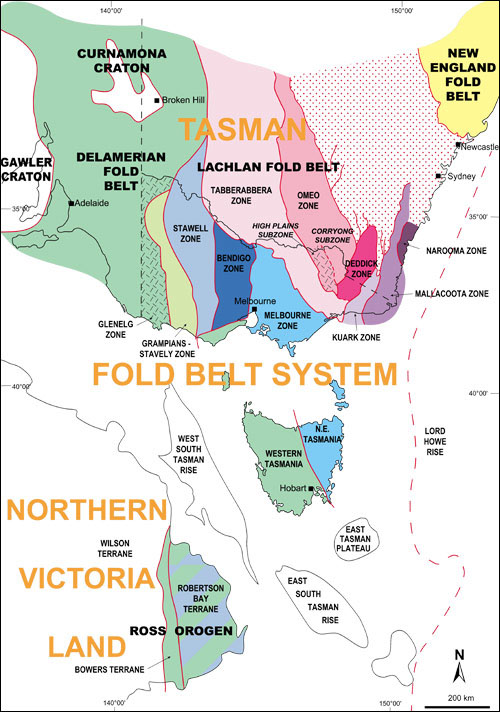
\includegraphics[width=1\textwidth]{Geology_Neoproterozoic_Fig_2.jpg}
\caption{\label{fig:VicStructuralZones}Map of eastern Australian fold belts and Victorian structural zones http://www.energyandresources.vic.gov.au/earth-resources/geology-of-victoria/geological-history/neo-car}
\end{figure}

\begin{figure}[H]
\centering
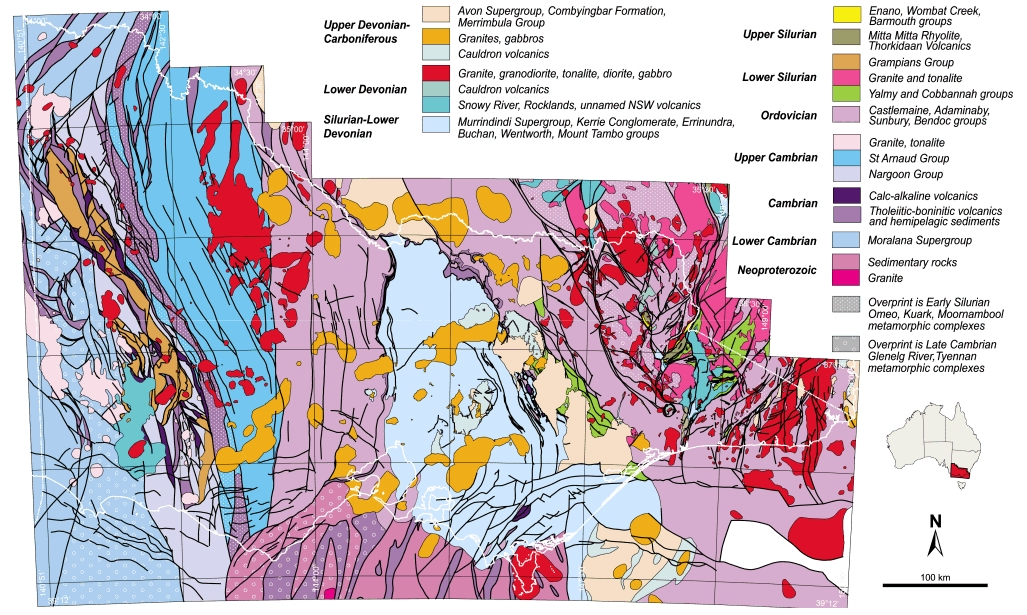
\includegraphics[width=1\textwidth]{vicmaprocktypes.jpg}
\caption{\label{fig:VicMapRockTypes}Description}
\end{figure}



\subsection{S-type}
S-type granites are composed of sedimentary rocks that have undergone anatexis.
Petrologically, they are more likely to contain meta-sedimentary xenoliths.S-type granites have a chemical composition that is relatively higher in sodium and calcium. It is thought that this distinction is the result of calcium enrichment in carbonate ans calcareous sediments and sodium enrichment through concentration on salt water and subsequent evaporation and capture as evaporitic sediments. 

\subsubsection{Chemical Composition}
Higher Sodium

\ce{Na2O} \textgreater 3.2\% in more felsic granites
t
\ce{Na2O} \textgreater 2.2\% in more mafic granites

Mol. \ce{Al2O3 / ( Na2O + K2O + CaO)} \textless 1.1

Higher Calcium

blah blah as above

\subsection{I type}
I-types granites are derived from igneous source material. Petrologically, they often contain mafic hornblende-bearing xenoliths

\subsubsection{Chemical Composition}
Lower Sodium

\ce{Na2O} \textless 3.2\% in more felsic granites

\ce{Na2O} \textless 2.2\% in more mafic granites

Mol. \ce{Al2O3 // ( Na2O + K2O + CaO)} \textgreater 1.1

\subsection{High and Low Temperature Granites}
Because felsic granites have similar major element geochemistry, a newer classification for the granites of Victoria has been proposed by Chappell, Bryant, etc and is temperature based. This classification utilises trace element geochemistry. As an example, S-type granites have high P and low Th and Ce relative abundance, compared to I-types \cite{chappell1998high}. Despite this classification system being different to S and I type granites, the higher temperature granites are generally classified as A type granites (felsic composition) or I type granites (mafic composition). Lower temperature granites being classified as S type and the remaining I type granites. These comprise \textasciitilde 90 \% of the Lachlan fold belt. \cite{chappell2001two}

\subsection{The Geological Setting}

It h
\begin{figure}[H]
\centering
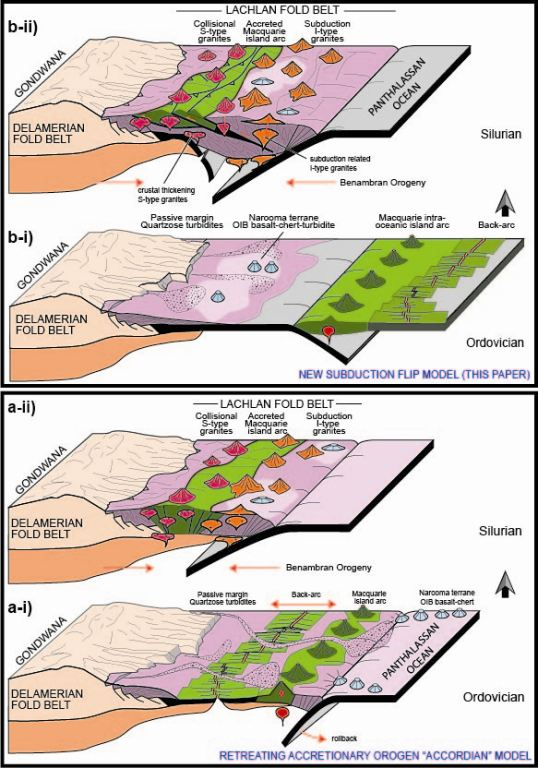
\includegraphics[width=1\textwidth]{granite_models.jpg}
\caption{\label{fig:GraniteModels} Possible formation models}
\end{figure}




\begin{figure}[H]
\centering
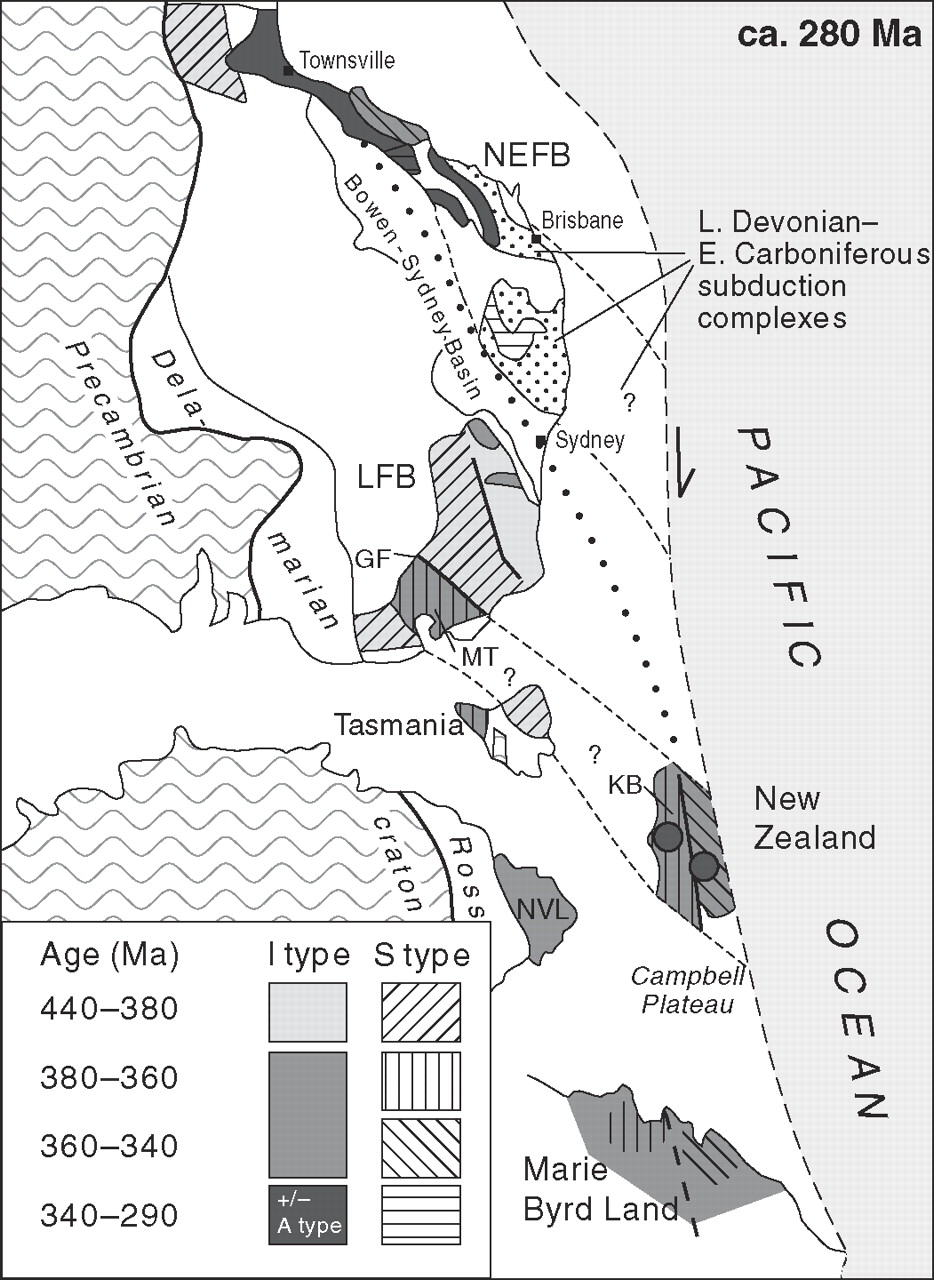
\includegraphics[width=1\textwidth]{Granite_Types_from_the_Eastern_Australian_Margin.jpg}
\caption{\label{fig:GraniteTypes}Granite Types from the Mesozoic Eastern Australian Margin}
\end{figure}

\begin{figure}[H]
\centering
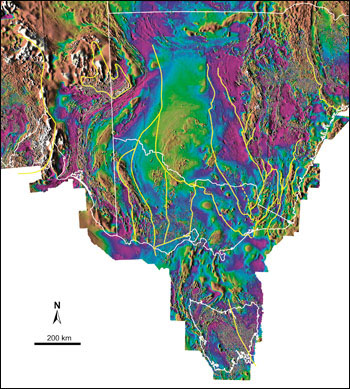
\includegraphics[width=1\textwidth]{Geology_Neoproterozoic_Fig_1.jpg}
\caption{\label{fig:mangneticImage}Regional magnetic image of southeastern Australia showing structural zone boundaries. Data sources: GSV, AGSO, PIRSA, MRT and GSNSW http://www.energyandresources.vic.gov.au/earth-resources/geology-of-victoria/geological-history/neo-car}
\end{figure}

\begin{figure}[H]
\centering
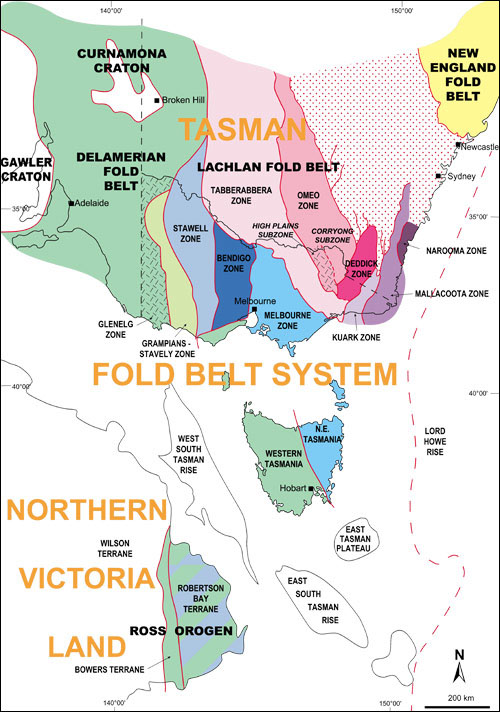
\includegraphics[width=1\textwidth]{Geology_Neoproterozoic_Fig_2.jpg}
\caption{\label{fig:
VicStructuralZones}Map of eastern Australian fold belts and Victorian structural zones http://www.energyandresources.vic.gov.au/earth-resources/geology-of-victoria/geological-history/neo-car}
\end{figure}
 



\section{Conclusion}

Conclusion


\newpage

\bibliography{bibliography.bib}

\end{document}